%
% IEEE Transactions on Microwave Theory and Techniques example
% Thibault Reveyrand - http://www.microwave.fr
%
% http://www.microwave.fr/LaTeX.html
% ---------------------------------------



% ================================================
% Please HIGHLIGHT the new inputs such like this :
% Text :
%  \hl{comment}
% Aligned Eq.
% \begin{shaded}
% \end{shaded}
% ================================================



\documentclass[journal]{IEEEtran}

%\usepackage[retainorgcmds]{IEEEtrantools}
%\usepackage{bibentry}
\usepackage{xcolor,soul,framed} %,caption

\colorlet{shadecolor}{yellow}
% \usepackage{color,soul}
\usepackage[pdftex]{graphicx}
\graphicspath{{../pdf/}{../jpeg/}}
\DeclareGraphicsExtensions{.pdf,.jpeg,.png}

\usepackage[cmex10]{amsmath}
%Mathabx do not work on ScribTex => Removed
%\usepackage{mathabx}
\usepackage{array}
\usepackage{mdwmath}
\usepackage{mdwtab}
\usepackage{eqparbox}
\usepackage{url}


% ----------------------------------------------

% Definitions of languages: ------------
\usepackage{listings}
\lstdefinestyle{cStyle}{
  basicstyle=\scriptsize,
  breakatwhitespace=false,
  breaklines=true,
  captionpos=b,
  keepspaces=true,
  numbersep=5pt,
  showspaces=false,
  gobble=4,
  tabsize=4,
  showstringspaces=false,
  showtabs=false,
}
\renewcommand*{\lstlistingname}{Code}

% ----------------------------------------------




\hyphenation{op-tical net-works semi-conduc-tor}

%\bstctlcite{IEEE:BSTcontrol}


%=== TITLE & AUTHORS ====================================================================
\begin{document}
\bstctlcite{IEEEexample:BSTcontrol}
    \title{Otimizations Based on Evolutionary Methods}
  \author{Carlos~Matheus~Barros~da~Silva,~\IEEEmembership{Bachelor Student of ITA}\\Prof. Marcos~Ricardo~Omena~de~Albuquerque~Máximo}


% The paper headers
\markboth{INSTITUTO TECNOLÓGICO DE AERONÁUTICA, APRIL~2019
}{Otimizations Based on Evolutionary Methods}


% ====================================================================
\maketitle



% === ABSTRACT ==============================================================
% ============================================================================
\begin{abstract}
%\boldmath
In this paper is evaluated an \texit{Evolutionary Optimization Method} denominated \texit{Simple Evolution Strategy} (SES) and its performance is compared with the \texit{Covariance Matrix Adaptation Evolution Strategy} (CMA-ES).

The results shows that since the SES approach not so sofisticated it needs a larger population in order to achieve as good resuls as CMA-ES gets with a smaller population.

Although in some cases they performed similary, and with a small increase in population in SES makes it perform as good as CMA-ES, and in some cases SES with a larger population performed better then CMA-ES. With this, therefore, SES is a simple and effective optimization method.

% === KEYWORDS ===============================================================
% ============================================================================
\begin{IEEEkeywords}
    Simple Evolution Strategy, SES, Covariance Matrix Adaptation Evolution Strategy, CMA-ES, optimization
\end{IEEEkeywords}

\IEEEpeerreviewmaketitle

% ====================================================================
% ====================================================================
% ====================================================================


% === I. INTRODUCTION ========================================================
% =============================================================================
\section{Introduction}

\IEEEPARstart{I}{n} computer science, an evolution strategy (ES) is an optimization technique based on ideas of evolution. It belongs to the general class of evolutionary computation or artificial evolution methodologies.

Usualy Evolution strategies use natural problem-dependent representations, and primarily mutation and selection, as search operators. In common with evolutionary algorithms, the operators are applied in a loop. An iteration of the loop is called a generation. The sequence of generations is continued until a termination criterion is met.

\subsection{Simple Evolution Strategy}

In this paper the \texit{Simple Evolution Strategy} (SES) approach relies on a covariance matrix and an mean. For each itetation, the algorithm makes a uniform sampling with the mean and covariance matrix and then gets the $\mu$ best positions and makes the mean of its position be the next mean, and uptate the covariance matrix. This SES behavior can be described with the Equation \ref{equation:esemean} and Equation \ref{equation:eseconvariancematrix}.

\begin{equation}
    \label{equation:esemean}
    m^{g+1} = \frac{1}{\mu} \sum_{i=1}^{\mu} S_{i:\lambda}^{g+1}
\end{equation}

\begin{equation}
    \label{equation:eseconvariancematrix}
    C^{g+1} = \frac{1}{\mu} \sum_{i=1}^{\mu} (S_{i:\lambda}^{g+1} - m^g) (S_{i:\lambda}^{g+1} - m^g)^T
\end{equation}

\subsection{Covariance Matrix Adaptation Evolution Strategy}

CMA-ES stands for covariance matrix adaptation evolution strategy. Evolution strategies (ES) are stochastic, derivative-free methods for numerical optimization of non-linear or non-convex continuous optimization problems. They belong to the class of evolutionary algorithms and evolutionary computation. An evolutionary algorithm is broadly based on the principle of biological evolution, namely the repeated interplay of variation (via recombination and mutation) and selection: in each generation (iteration) new individuals (candidate solutions, denoted as $x$) are generated by variation, usually in a stochastic way, of the current parental individuals. Then, some individuals are selected to become the parents in the next generation based on their fitness or objective function value $f(x)$. Like this, over the generation sequence, individuals with better and better $f$-values are generated.

In an evolution strategy, new candidate solutions are sampled according to a multivariate normal distribution in ${R}^{n}$. Recombination amounts to selecting a new mean value for the distribution. Mutation amounts to adding a random vector, a perturbation with zero mean. Pairwise dependencies between the variables in the distribution are represented by a covariance matrix. The covariance matrix adaptation (CMA) is a method to update the covariance matrix of this distribution. This is particularly useful if the function $f$ is ill-conditioned.

Adaptation of the covariance matrix amounts to learning a second order model of the underlying objective function similar to the approximation of the inverse Hessian matrix in the Quasi-Newton method in classical optimization. In contrast to most classical methods, fewer assumptions on the nature of the underlying objective function are made. Only the ranking between candidate solutions is exploited for learning the sample distribution and neither derivatives nor even the function values themselves are required by the method.

Two main principles for the adaptation of parameters of the search distribution are exploited in the CMA-ES algorithm.

First, a maximum-likelihood principle, based on the idea to increase the probability of successful candidate solutions and search steps. The mean of the distribution is updated such that the likelihood of previously successful candidate solutions is maximized. The covariance matrix of the distribution is updated (incrementally) such that the likelihood of previously successful search steps is increased. Both updates can be interpreted as a natural gradient descent. Also, in consequence, the CMA conducts an iterated principal components analysis of successful search steps while retaining all principal axes. Estimation of distribution algorithms and the Cross-Entropy Method are based on very similar ideas, but estimate (non-incrementally) the covariance matrix by maximizing the likelihood of successful solution points instead of successful search steps.

Second, two paths of the time evolution of the distribution mean of the strategy are recorded, called search or evolution paths. These paths contain significant information about the correlation between consecutive steps. Specifically, if consecutive steps are taken in a similar direction, the evolution paths become long. The evolution paths are exploited in two ways. One path is used for the covariance matrix adaptation procedure in place of single successful search steps and facilitates a possibly much faster variance increase of favorable directions. The other path is used to conduct an additional step-size control. This step-size control aims to make consecutive movements of the distribution mean orthogonal in expectation. The step-size control effectively prevents premature convergence yet allowing fast convergence to an optimum.

% ==========================================================================
\section{Simple Evolution Strategy (SES) Implementation}

The implementation was b

The implementation was based on the file \textit{particle swarm optimization}. The essence is on \textit{ParticleSwarmOptimization} Class and \textit{Particle} Class development. The first one provides the interface in which the simulation communicates with the PSO.

Based on this, the development of \textit{ParticleSwarmOptimization} Class was oriented to receive inputs, provides information, and have methods that trigger the algorithm continuation.

In order to achieve this, it was developed the methods shown from the Code \ref{code:particle_swarm_optimization} to the Code \ref{code:notify_evaluation}.

\lstinputlisting[
    language=python,
    caption={Constructor of \textit{PSO} Class.},
    label={code:particle_swarm_optimization},
    style=cStyle,
    firstline=78,
    lastline=85
]{./../code/particle_swarm_optimization.py}

\lstinputlisting[
    language=python,
    caption={Method \textit{get best position} of \textit{PSO} Class.},
    label={code:get_best_position},
    style=cStyle,
    firstline=93,
    lastline=94
]{./../code/particle_swarm_optimization.py}

\lstinputlisting[
    language=python,
    caption={Method \textit{get best value} of \textit{PSO} Class.},
    label={code:get_best_value},
    style=cStyle,
    firstline=101,
    lastline=101
]{./../code/particle_swarm_optimization.py}

\lstinputlisting[
    language=python,
    caption={Method \textit{get position to evaluate} of \textit{PSO} Class.},
    label={code:get_position_to_evaluate},
    style=cStyle,
    firstline=110,
    lastline=111
]{./../code/particle_swarm_optimization.py}

\lstinputlisting[
    language=python,
    caption={Method \textit{advance generation} of \textit{PSO} Class.},
    label={code:advance_generation},
    style=cStyle,
    firstline=117,
    lastline=120
]{./../code/particle_swarm_optimization.py}

\lstinputlisting[
    language=python,
    caption={Method \textit{notify evaluation} of \textit{PSO} Class.},
    label={code:notify_evaluation},
    style=cStyle,
    firstline=129,
    lastline=141
]{./../code/particle_swarm_optimization.py}

The two main methods during the execution are the \textit{get position to evaluate} that returns to simulation the position of one particle, and the \textit{nofify evalutation} that gives the simulation result of that position to the \textit{PSO} algorithm. With the result, the code checks if it is the best of that specific particle, or if it is the best overall. Then advance the index to next iteration.

This advance index step is quite important, bacause if the index reaches the population size, it calls the method \textit{advance generation} that will update the velocity and the position of every particle and reset the index.

\subsection {Particle Class Implementation}

Objects of this class store its position, its velocity, and its best position. The class provides, as well, methods to the particle update its velocity and its position.

The implementation of Particle Class is shown from Code \ref{code:particle} to Code \ref{code:update_particle_position}.

\lstinputlisting[
    language=python,
    caption={Constructor of \textit{Particle} Class.},
    label={code:particle},
    style=cStyle,
    firstline=19,
    lastline=41
]{./../code/particle_swarm_optimization.py}

\lstinputlisting[
    language=python,
    caption={Method \textit{update particle velocity} of \textit{PSO} Class.},
    label={code:update_particle_velocity},
    style=cStyle,
    firstline=43,
    lastline=51
]{./../code/particle_swarm_optimization.py}

\lstinputlisting[
    language=python,
    caption={Method \textit{update particle position} of \textit{PSO} Class.},
    label={code:update_particle_position},
    style=cStyle,
    firstline=53,
    lastline=59
]{./../code/particle_swarm_optimization.py}

\subsubsection{Update velocity}

The \texit{updatae velocity} method uses Equation \ref{equation:update_velocity}. Where $r_p$ and $r_g$ are two different random numbers between 0 and 1 generated on every time the equation is calculated.

The $\phi_p$ is called the congnitve parameter, and it is a constant that multiplies the vector $(b_i - x_i)$ which is the direction to the best position of that particle.

The $\phi_g$ is called the social parameter, and it is a constant that multiplies the vector $(b_g - x_i)$ which is the direction to the best position in all particles.

Therefore the constants $\phi_p$ and $\phi_g$ balance how much importance will be the best position locally and the best position globally.

Basicly this is a balance between explorateion and explotation. The bigger the importancy of the global best, the more proprable to converge to a not so good local maximum. The bigger the importancy of local best, the more problable to find a better solution, but with a more slow convergency.

\begin{equation}
    \label{equation:update_velocity}
    v_{i+1} = \omega v_i + \phi_p r_p (b_i - x_i) + \phi_g r_g (b_g - x_i)
\end{equation}

\subsubsection {Update position}

In order to update the particle position. Its current position is added to its calculated new velocity. This can is seen in the Code \ref{code:update_particle_position}.

As professor Maximo suggested during his lecture, it was implemented a particle reflection, when one of them fall out of the bounderies while updating its position.

\section{PSO result in test function}

As suggested, the PSO implementation was first tested using an easy test function in order to verify its correctness.

The cost function used in the test was described on Equation \ref{equation:test_fuction}, in which has a global maximum $[1 2 3]$.

\begin{equation}
    \label{equation:test_fuction}
    f(x, y, z) = -((x - 1)^2 + (y-2)^2 + (z-3)^2)
\end{equation}

In tests conducted usin 40 particles and 1000 generations, the PSO converged rapdly to the global maximum. The position an quality of the results can be seen in Code \ref{code:position_test_function} and Code \ref{code:quality_test_function}.

\lstinputlisting[
    language=python,
    caption={Positions results on Test function, shown only the first 10 and the last 10.},
    label={code:position_test_function},
    style=cStyle,
]{./../code/test_function_result/test_short_position_history.txt}

\lstinputlisting[
    language=python,
    caption={Quality result on Test function, shown only the first 10 and the last 10},
    label={code:quality_test_function},
    style=cStyle,
]{./../code/test_function_result/test_short_quality_history.txt}

It is possible to see with the Figure \ref{img:test_best_quality_converge} to Figure \ref{img:test_parameters_quality_converge}, the convergency on the best position, the overall converge, and the converge of the parameters.

\begin{figure}
  \begin{center}
  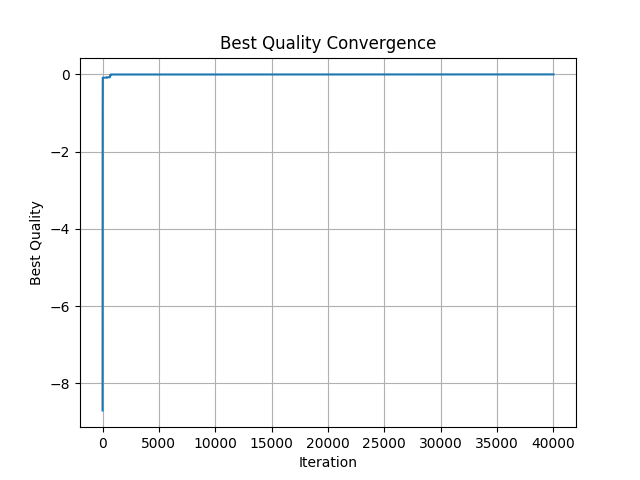
\includegraphics[width=2.8in]{./../code/test_function_result/test_best_convergence.png}
  %\vspace{-15pt}
  \caption{Test best quality convergency}
  \label{img:test_best_quality_converge}
  \end{center}
\end{figure}

\begin{figure}
  \begin{center}
  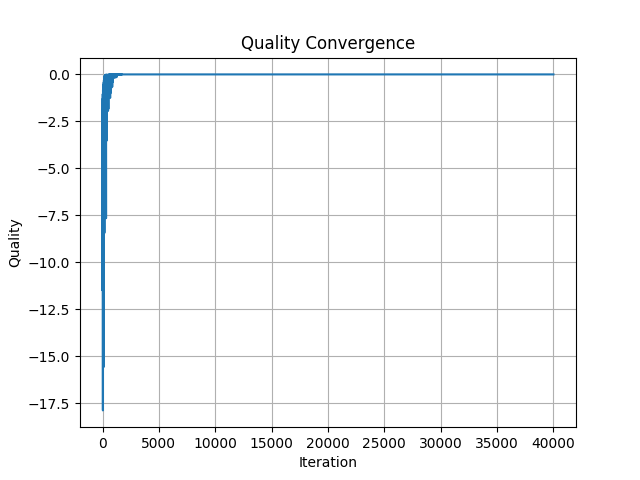
\includegraphics[width=2.8in]{./../code/test_function_result/test_quality_converge.png}
  %\vspace{-15pt}
  \caption{Test quality convergency}
  \label{img:test_quality_converge}
  \end{center}
\end{figure}

\begin{figure}
  \begin{center}
  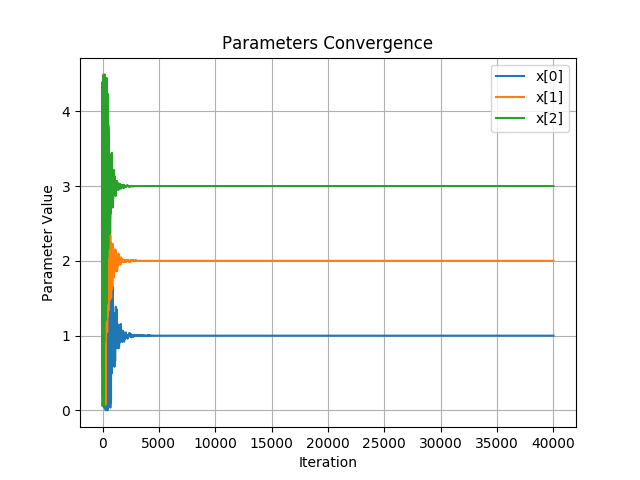
\includegraphics[width=2.8in]{./../code/test_function_result/test_parameters_converge.png}
  %\vspace{-15pt}
  \caption{Test parameters convergency}
  \label{img:test_parameters_quality_converge}
  \end{center}
\end{figure}

Thus it is clear that the algorithm works and converges accordingly. That said, the algorithm is ready to be used on the line follower problem.

\section {PSO on Line Follower Problem}

From a car circuit simulation, it was developed a line follower opmization on the \textit{proportional–integral–derivative controller (PID controller)} Control technique.

From the Equation \ref{equation:control_equation}, the objectve of this optimization is to optimize $K_p$, $K_i$, $K_d$, and the linear velocity of the car.

\begin{equation}
    \label{equation:control_equation}
    u(t) =  K_p e(t) + K_i \int_{0}^{t} e(t')dt'+K_d \frac{de(t)}{dt}
\end{equation}

In order to do that, the \textit{PSO} algorithm was run with 40 particles and it was developed the \textit{evaluate} method. With this method, every position of the car was evaluated and the sum of all evaluations was the score of the position of that particle.

The \textit{evaluate} method can be seen in the Code \ref{code:evaluate}, where by the end of the implementation was defined a high weight on linear speed and severe penalty for high errors and miss the track.

\lstinputlisting[
    language=python,
    caption={Method \textit{evaluate} of \textit{Simulation} Class, it is intended atribute a score for the situation of a particle.},
    label={code:evaluate},
    style=cStyle,
    firstline=130,
    lastline=152
]{./../code/simulation.py}

In the firsts tests, it was clear that the convergency was always slow and always tending first to a quite slow velocity.

Therefore a higher weight was given to linear speed and the velocity upper bounder was increased.

\subsection{Concise convercency}

After the adjustment, the algorithm was run with 40 particles for about two hours, which resulted in 5477 iterations.

The quality history and the position history can be seen in the Code \ref{code:position_pso} and Code \ref{code:quality_pso}.

The convergencies can be seen in the figures from Figure \ref{img:best_quality_converge} to Figure \ref{img:quality_converge}.

\lstinputlisting[
    language=python,
    caption={Positions results on PSO optimization, shown only the first 10 and the last 10.},
    label={code:position_pso},
    style=cStyle,
]{./../code/results/short_position_history.txt}

\lstinputlisting[
    language=python,
    caption={Quality result on PSO optimization, shown only the first 10 and the last 10},
    label={code:quality_pso},
    style=cStyle,
]{./../code/results/short_quality_history.txt}

\begin{figure}
  \begin{center}
  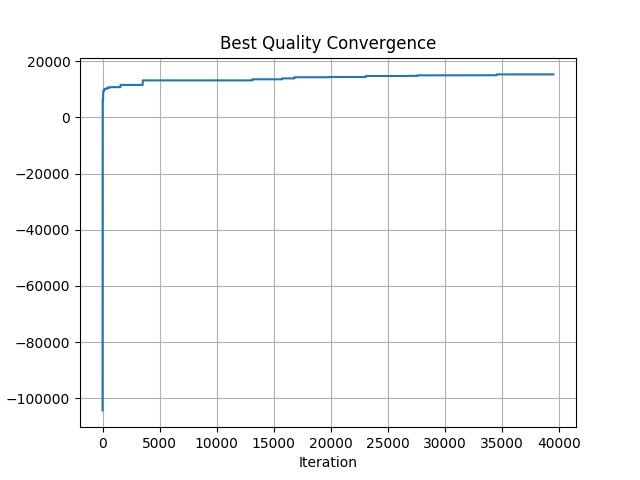
\includegraphics[width=2.8in]{./../code/results/line_best_convergence.png}
  %\vspace{-15pt}
  \caption{Best quality convergency}
  \label{img:best_quality_converge}
  \end{center}
\end{figure}

\begin{figure}
  \begin{center}
  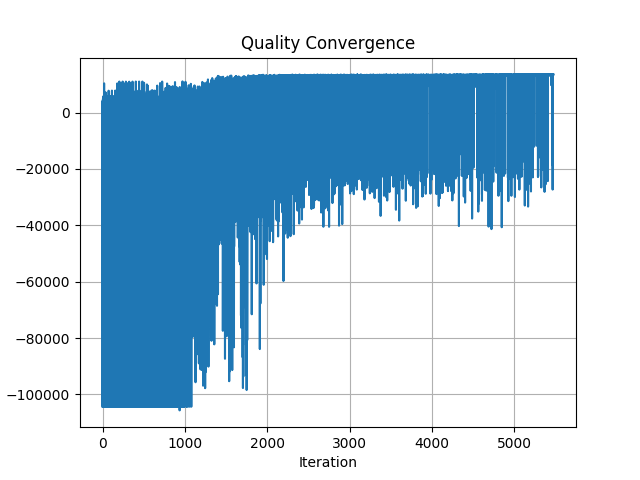
\includegraphics[width=2.8in]{./../code/results/line_quality_convergence.png}
  %\vspace{-15pt}
  \caption{Quality convergency}
  \label{img:quality_converge}
  \end{center}
\end{figure}

\begin{figure}
  \begin{center}
  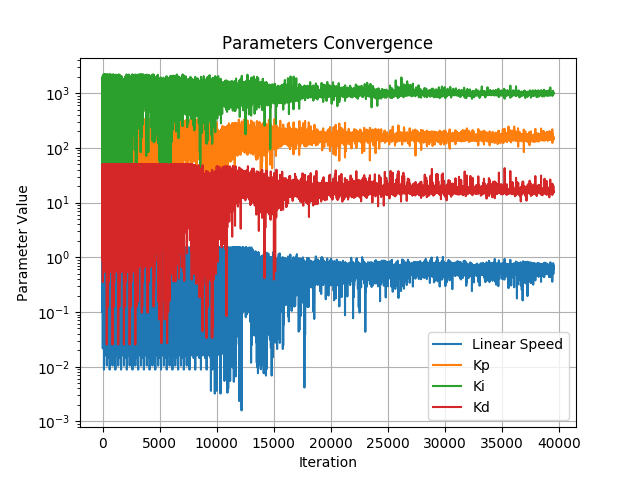
\includegraphics[width=2.8in]{./../code/results/line_parameters_convergence.png}
  %\vspace{-15pt}
  \caption{Parameters convergency}
  \label{img:parameters_quality_converge}
  \end{center}
\end{figure}

\section {Conclusion}

It was clear, therefore, that \textit{PSO} method was implemented successfully. And by analyzing its results, it can be seen that \textit{PSO} has a fast conversion, but it does not converge to something necessarily great.

In fact, it finds local maximums and can easily be stocked on it. But for many cases, it is good enough. In the case test, the solution found was able to complete the entire track in about 11 seconds, that is, it was really fast and precise at the same time.

As it is possible to see on the on Figure \ref{img:initial_line_follower_solution} and Figure \ref{img:initial_line_follower_solution} that at initials iterations the parameters are really bad, and with the time after many iterations it has a convergence to something good.

\begin{figure}
  \begin{center}
  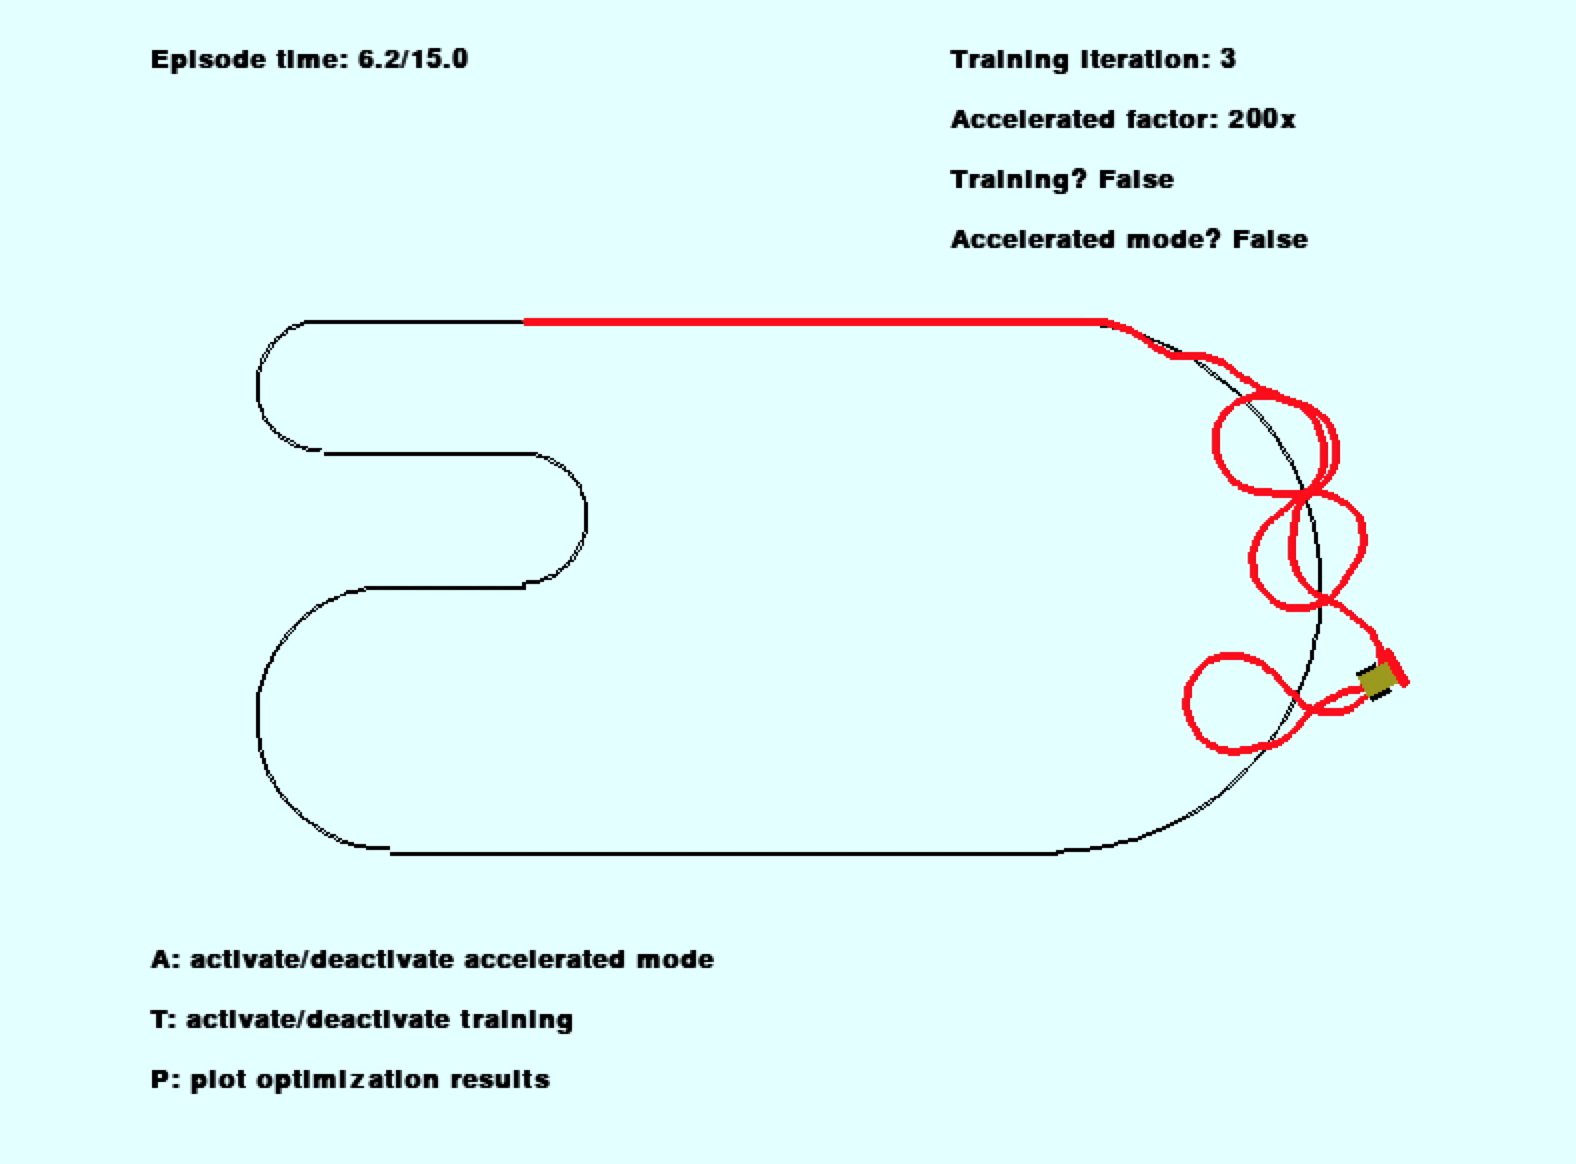
\includegraphics[width=2.8in]{./../code/results/initial_line_follower_solution.png}
  %\vspace{-15pt}
  \caption{Screenshot of the begging of the solution. Clearly the line follower was with bad parameter at this iteration.}
  \label{img:initial_line_follower_solution}
  \end{center}
\end{figure}

\begin{figure}
  \begin{center}
  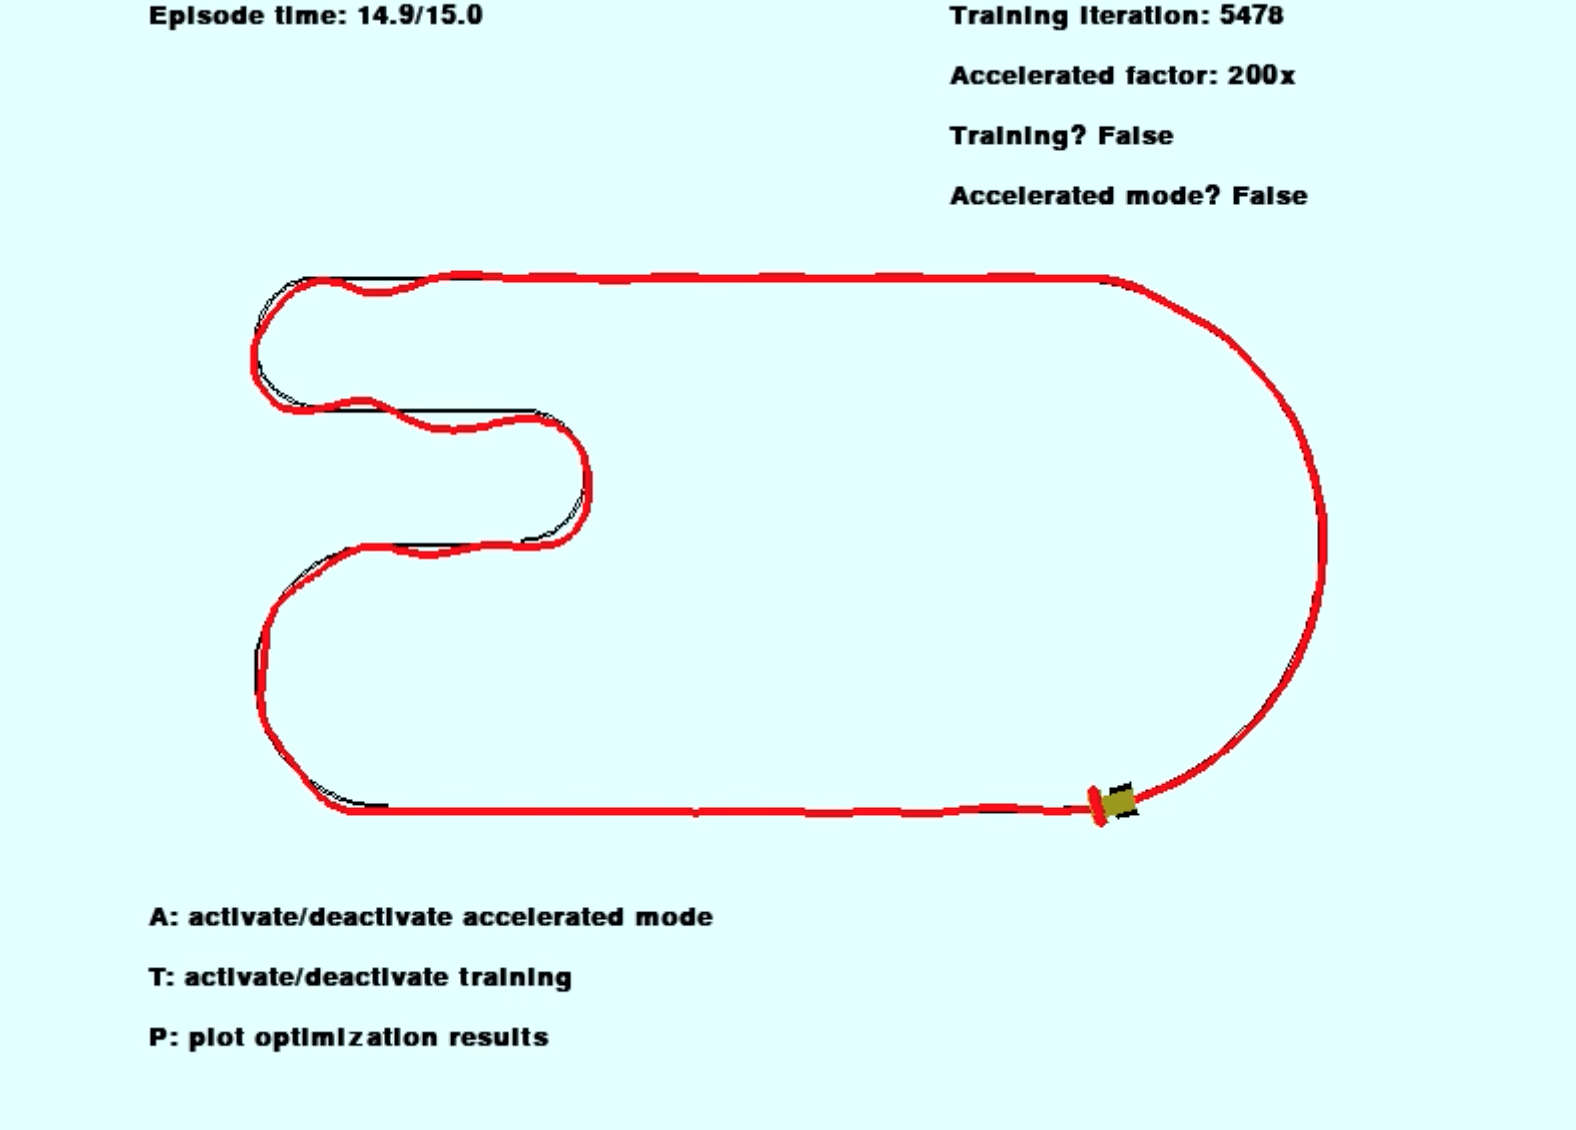
\includegraphics[width=2.8in]{./../code/results/line_follower_solution.png}
  %\vspace{-15pt}
  \caption{Screenshot at iteration number 5478. Clearly the line follower is now with good parameters.}
  \label{img:line_follower_solution}
  \end{center}
\end{figure}


\vfill
\end{document}
